\section{Tube selection}
At the very beginning, we simply chose a body with a plastic tube called 'Quantum'.
I have one of these tubes at home which is approximately 1.2 m tall. Since we had
to choose a height for the rocket, we decided to make it approximately 1 m tall,
including the motor, ailerons and nose.

\begin{figure}[!hbt]
    \centering
    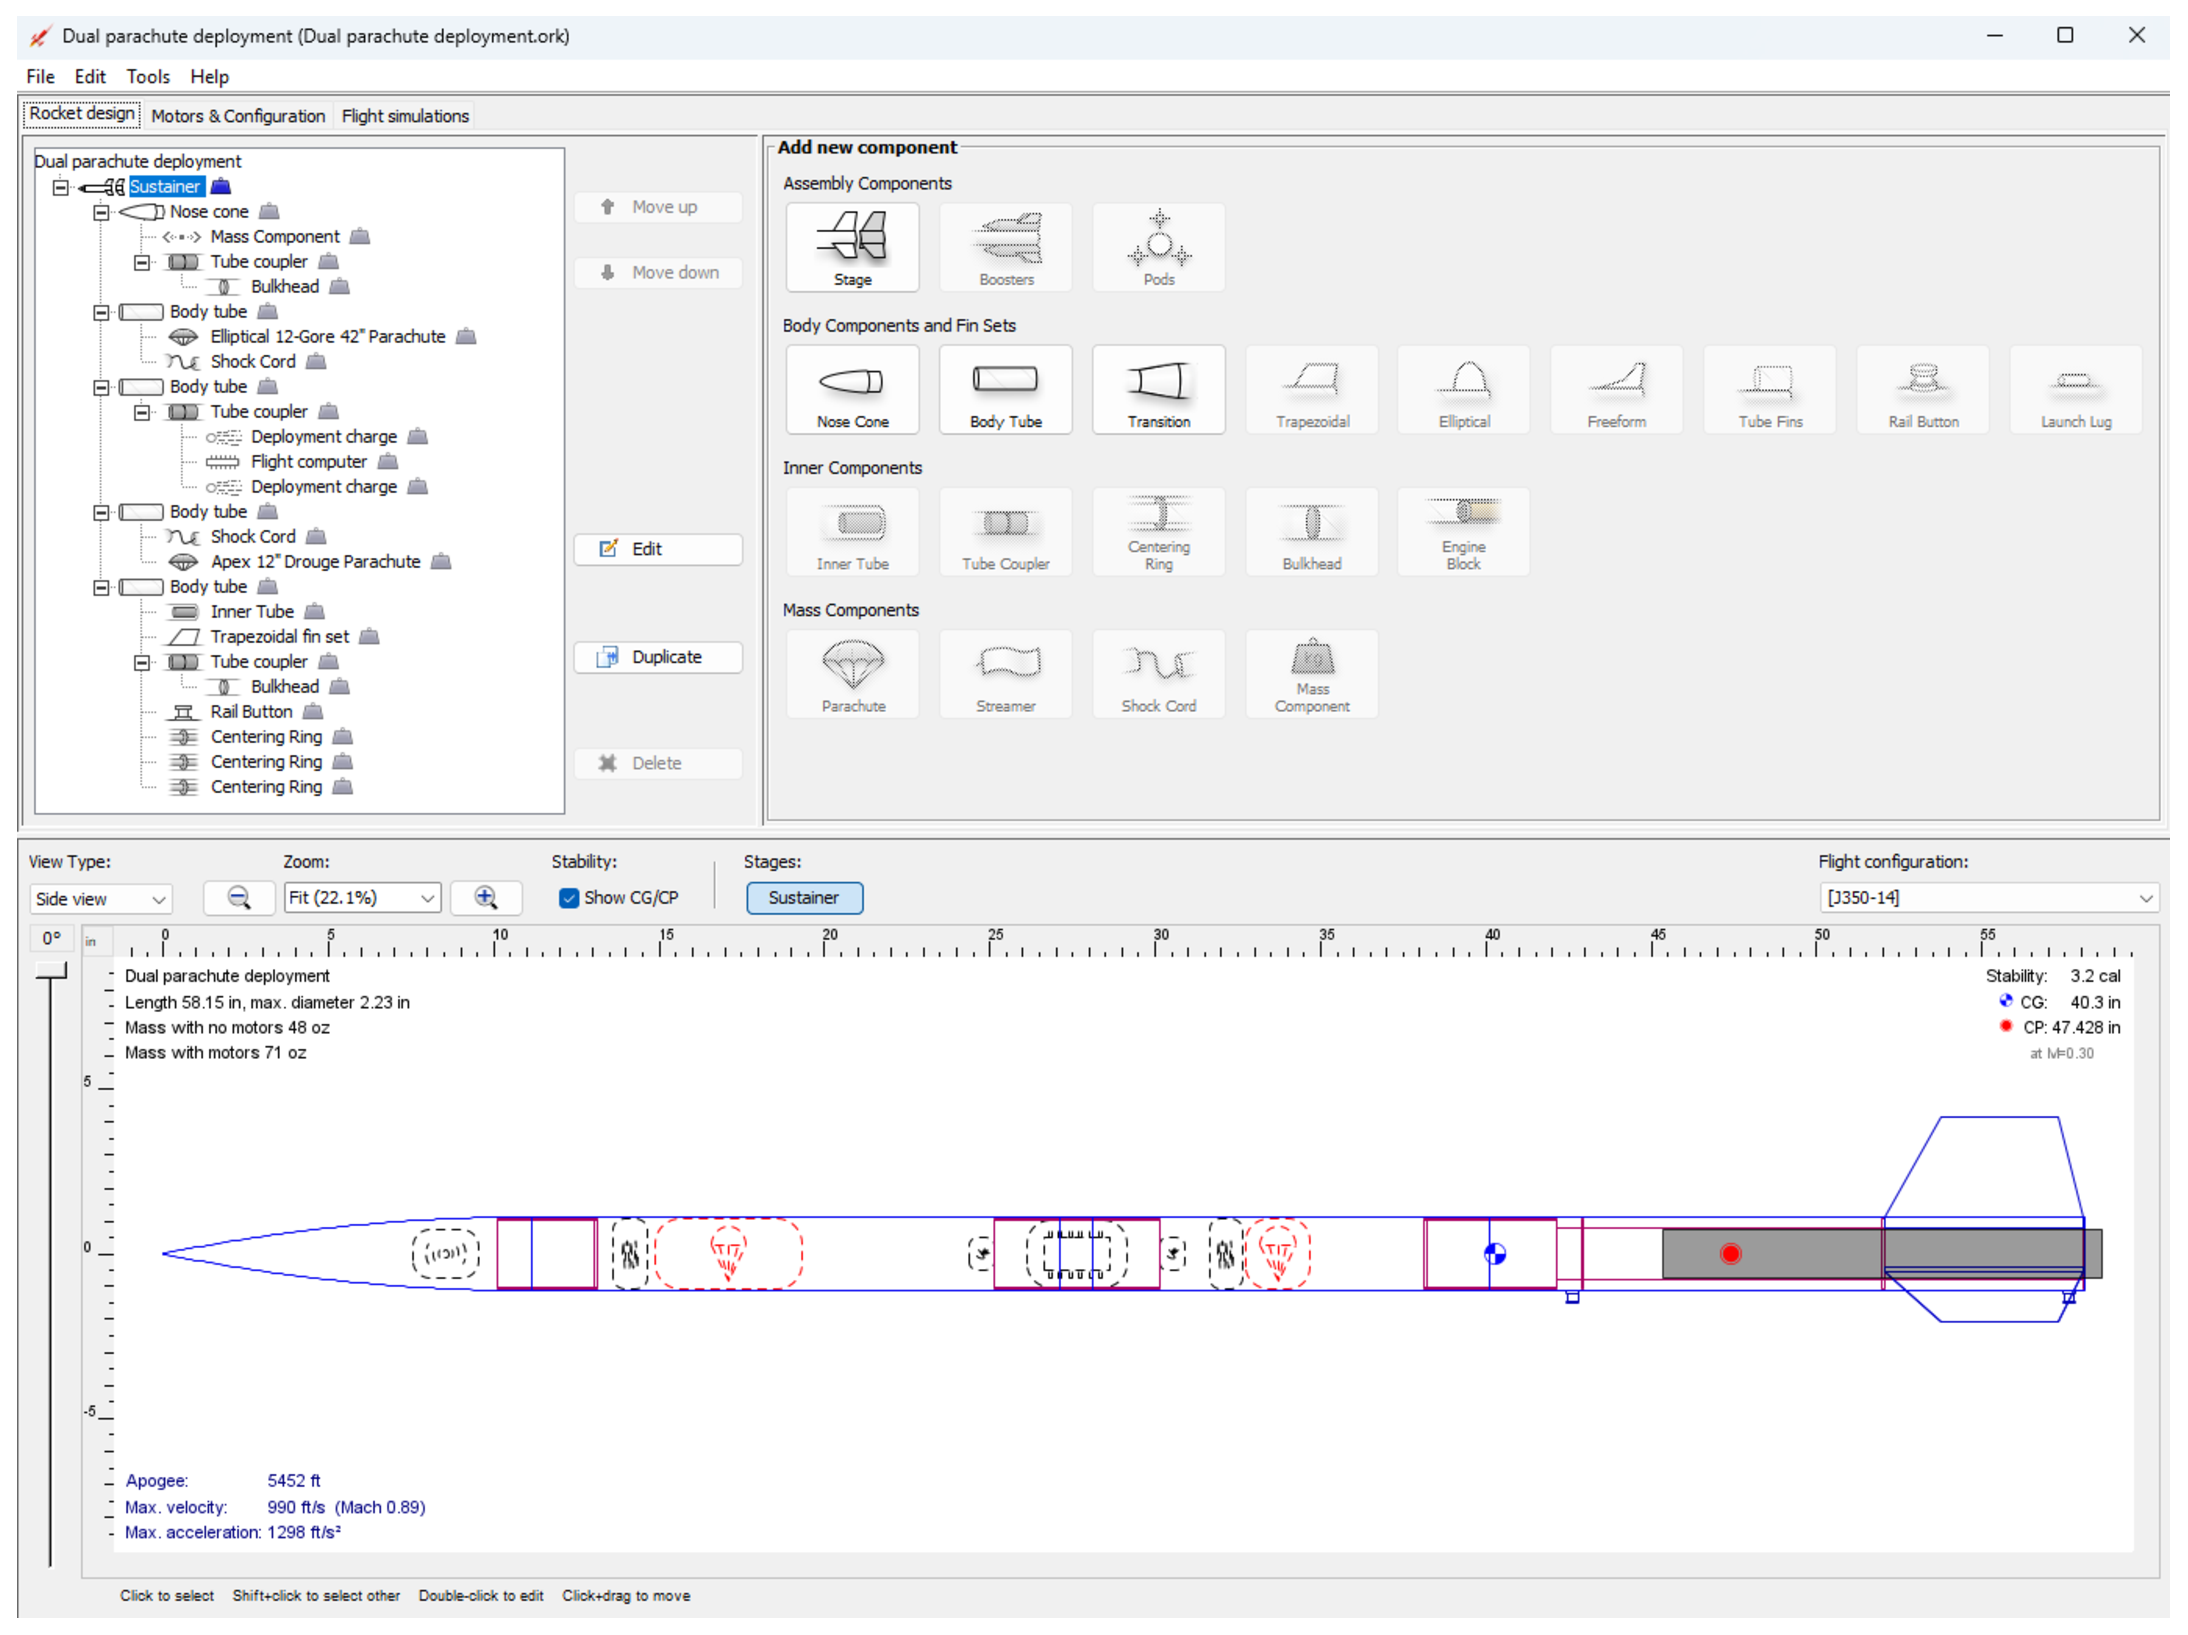
\includegraphics[width=\SchematicWidth]{\Images/mechanical/OpenRocket.eps}
    \caption{Screenshot of the tool used design and simulate rockets.}
\end{figure}
\FloatBarrier

\paragraph{}
One of the most important aspects of building a model rocket is the CG/CL ratio,
and this is something we had to consider. This ratio represents the division between
the position of the centre of gravity and the centre of lift. It represents the
rocket's inherent stability. Our centre of gravity needs to be in front of the
centre of lift, following the axis of our rocket body. The ratio needs to be at
least 1 for the rocket to be stable without an active stabilisation system.

\paragraph{}
For this project, we challenged ourselves by choosing to add active stabilisation
to our rocket in the form of ailerons for control surfaces. We positioned them at
the front of the rocket to maintain the stabilisation provided by the rear ailerons
while retaining control over the rocket's direction. Due to the complexity of the
equations, we chose to ignore the turbulence caused by the front ailerons on the
rear ailerons.

\paragraph{}
One issue arising from the front control ailerons is that they reduce the CG/CL
ratio, as we have added lift to the front of the rocket, thus advancing the CL.
This gave us a ratio of about 0.5, which is considered unstable. This would be
undesirable for a normal rocket, but because our rocket is actively stabilised,
we can afford this kind of trade-off.
We used Open Rocket to design the nose cone of the rocket, which gave us an idea
of the different types of nose cone used in model rockets. We chose the simplest
option: an ellipsoidal cone.

\paragraph{}
To keep things simple, we will 3D print the nose cone and use acetone to smooth
the outer part. We did the same for all eight ailerons and the four control and
static surfaces.

\paragraph{}
Another problem of our rocket is to hold the rocket motor. Our rocket is mostly
composed of plastic and so it will melt at the contact of the motor. We choose
cork which is very poor conductor of heat to hold our motor.

Every part we talked about is to be built in the near future and assembled.